\documentclass{beamer}
\usetheme{default}
\title{Hybrid ray tracer}
\date{\today}

\begin{document}
\begin{frame}
	\titlepage
\end{frame}
\begin{frame}
	Iterative ray tracer
	\begin{figure}
		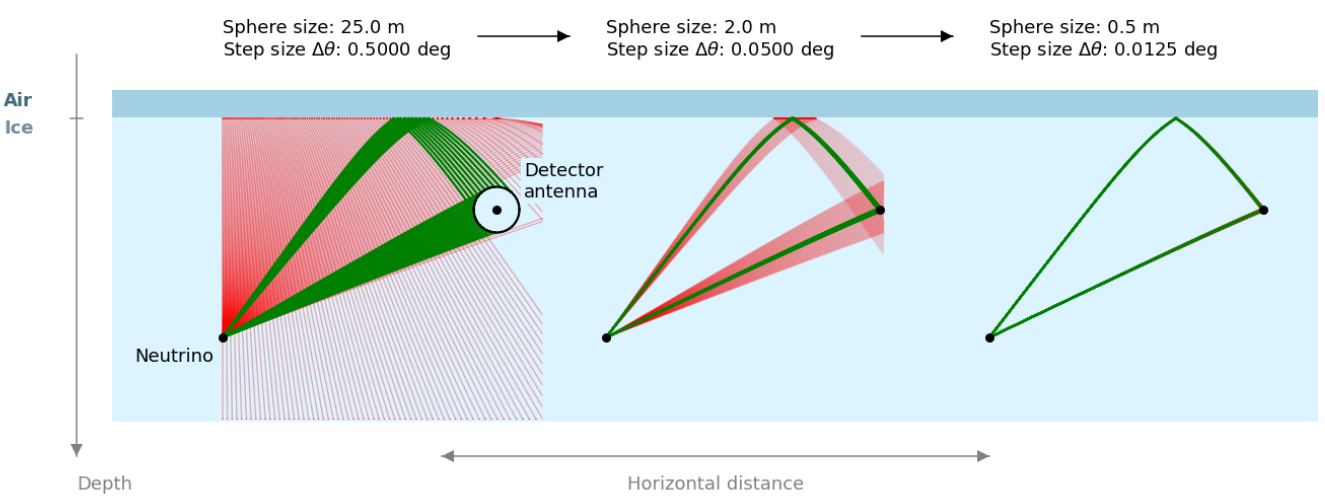
\includegraphics[width=\textwidth]{figures/iterative_explanation.png}
	\end{figure}
\end{frame}
\begin{frame}
	Python: Slow ($\approx 300$ Times the execution time of C++)\\
	Solution: scipy.optimize.minimize
\end{frame}
\begin{frame}
	\begin{figure}
		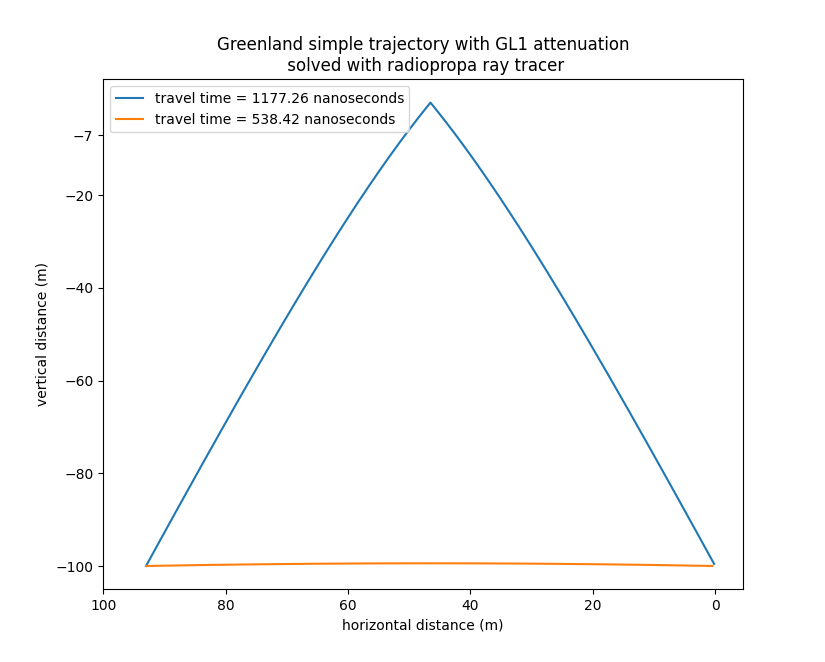
\includegraphics[width=\textwidth]{figures/iterative.png}
	\end{figure}
\end{frame}
\begin{frame}
	\begin{figure}
		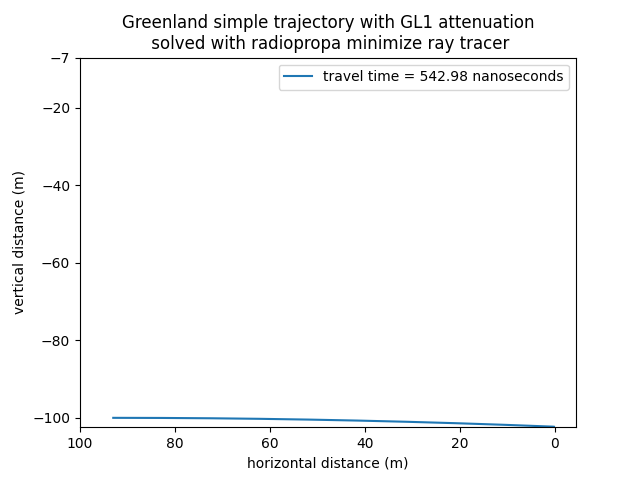
\includegraphics[width=\textwidth]{figures/minimize.png}
	\end{figure}
\end{frame}
\begin{frame}
	\begin{figure}
		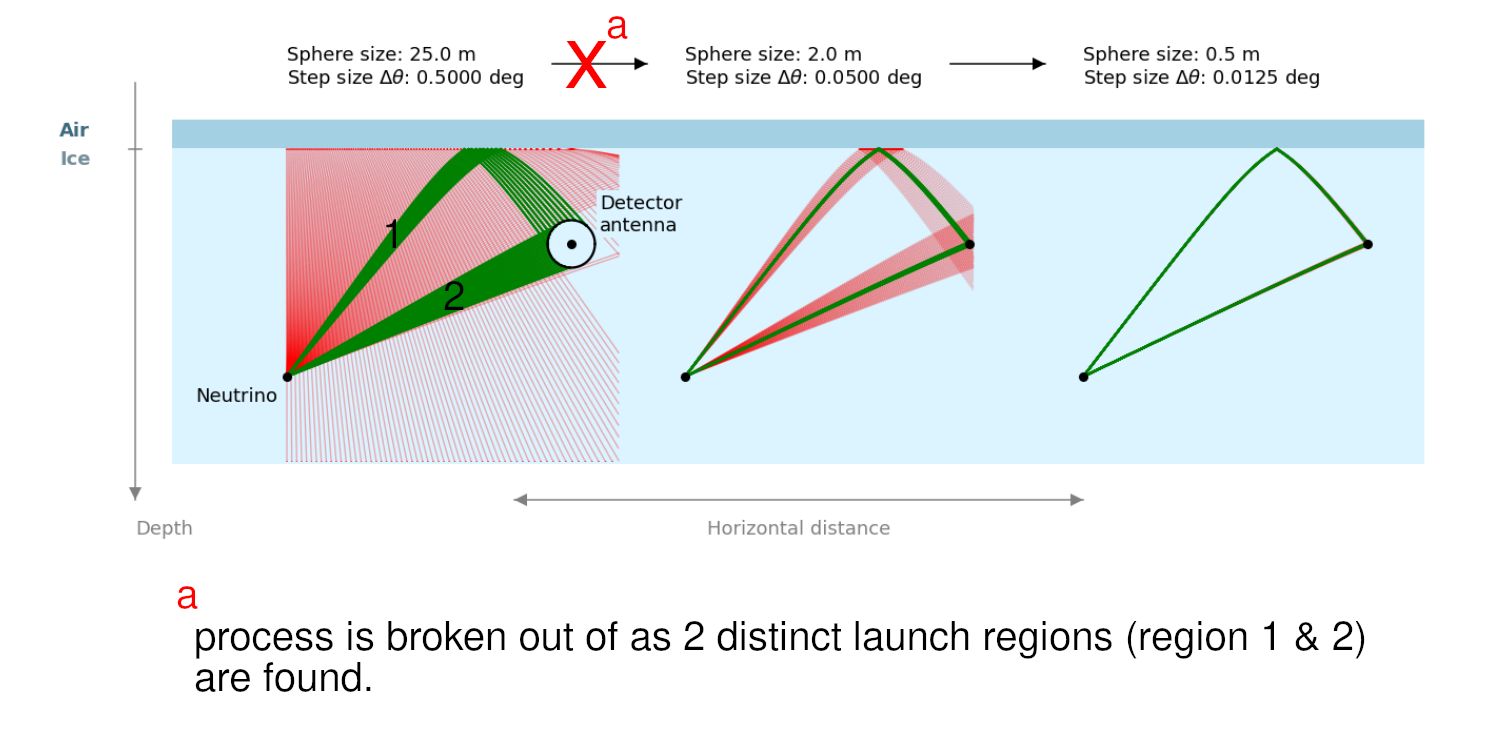
\includegraphics[width=\textwidth]{figures/explanation.png}
	\end{figure}
\end{frame}
\begin{frame}
	\begin{figure}
		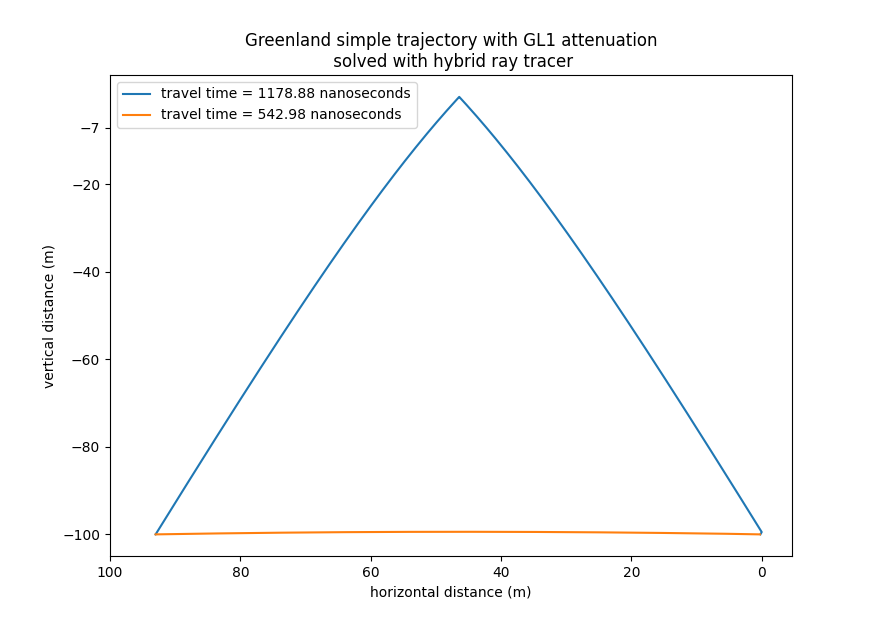
\includegraphics[width=\textwidth]{figures/hybrid.png}
	\end{figure}
\end{frame}
\begin{frame}
	\begin{figure}
		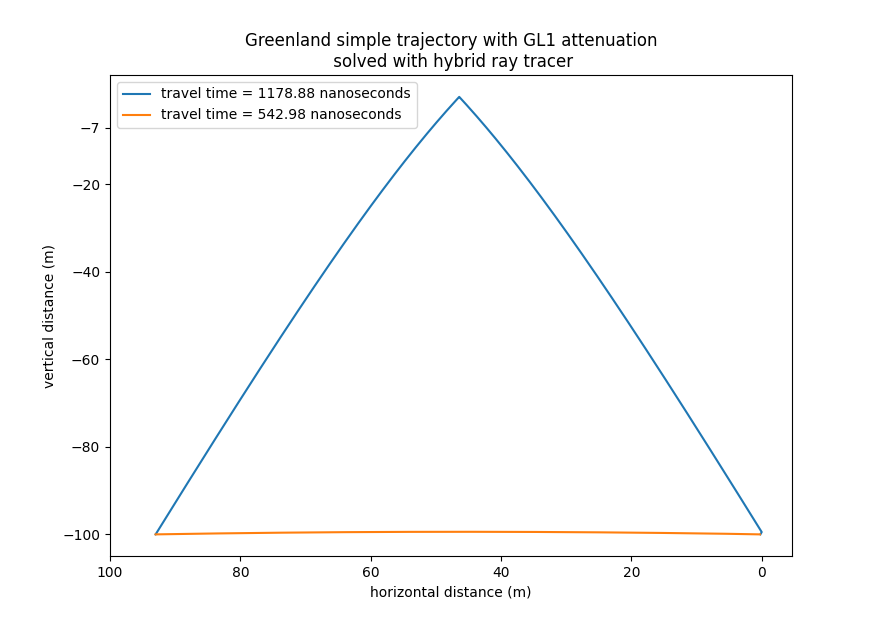
\includegraphics[width=\textwidth]{figures/hybrid.png}
	\end{figure}
\end{frame}
\begin{frame}
	\begin{figure}
		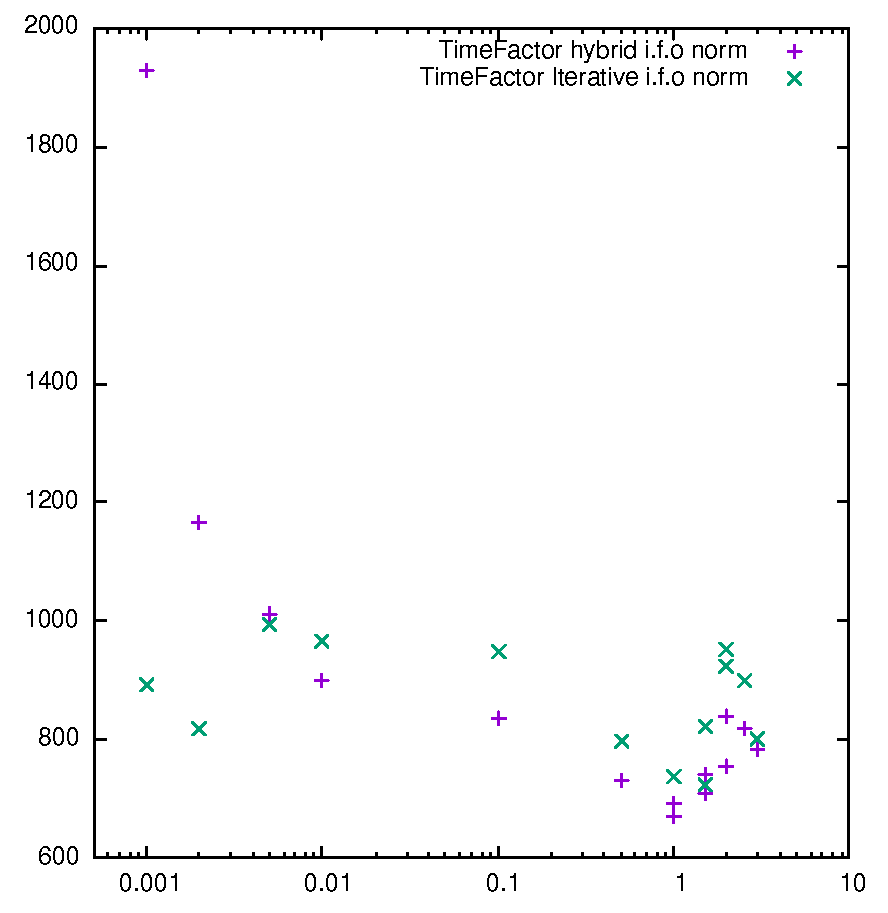
\includegraphics[width=0.7\textwidth]{figures/NormVsTime.pdf}
	\end{figure}
\end{frame}
\begin{frame}
	\begin{minipage}{0.49\textwidth}
	\begin{figure}
		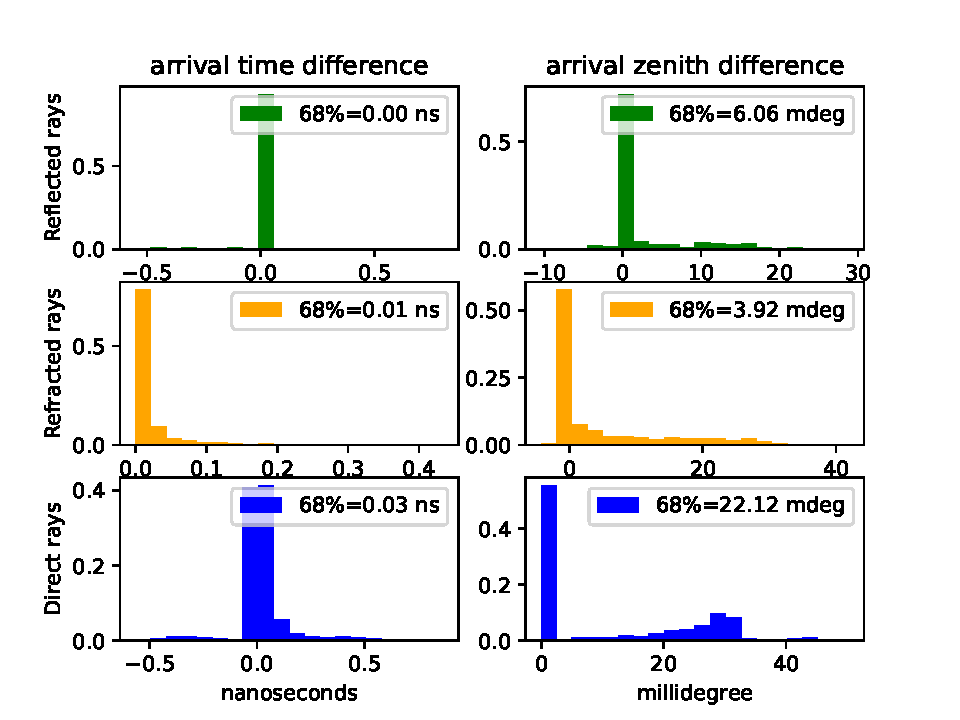
\includegraphics[width=1.1\textwidth]{figures/hybrid_comparison_N_1000.pdf}
		\caption{Hybrid}
	\end{figure}
	\end{minipage}
	\begin{minipage}{0.49\textwidth}
	\begin{figure}
		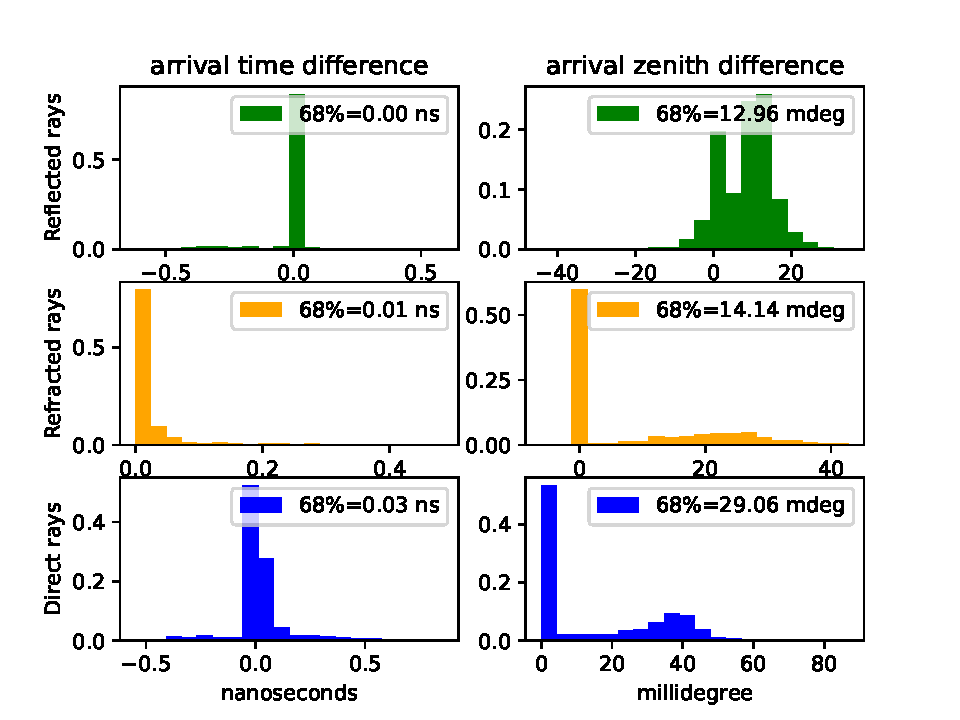
\includegraphics[width=1.1\textwidth]{figures/iterative_comparison_N_1000.pdf}
		\caption{Iterative}
	\end{figure}
	\end{minipage}
Whilst $\approx 10\%$ faster
\end{frame}
\end{document}
